\begin{frame}[fragile]{libraries}
\begin{Verbatim}[fontsize=\small]
$ objdump --all-headers mystery
\end{Verbatim}
\ldots
\begin{Verbatim}[fontsize=\small]
Dynamic Section:
  NEEDED               libncurses.so.6
  NEEDED               libtinfo.so.6
  NEEDED               libc.so.6
\end{Verbatim}
\ldots
\end{frame}

\begin{frame}[fragile]{ncurses?}
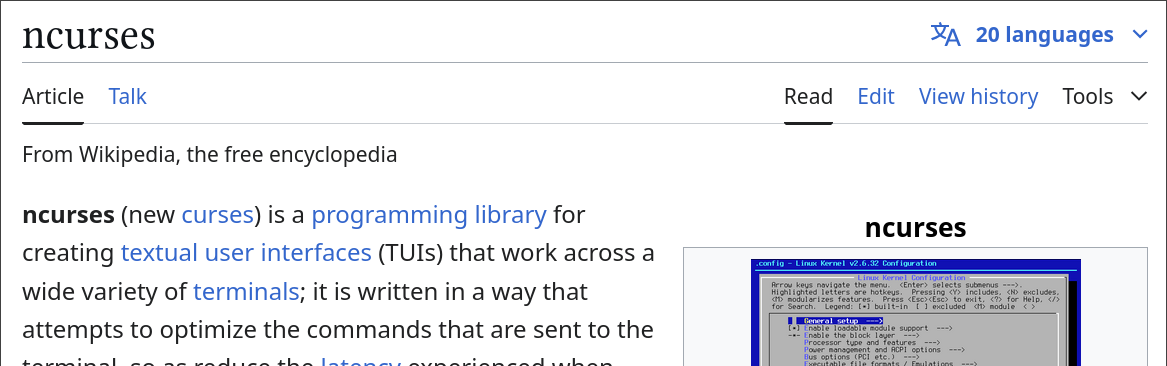
\includegraphics[width=\textwidth]{../re-tools/ncurses-wiki}
\end{frame}

\begin{frame}[fragile]{tinfo? (1)}
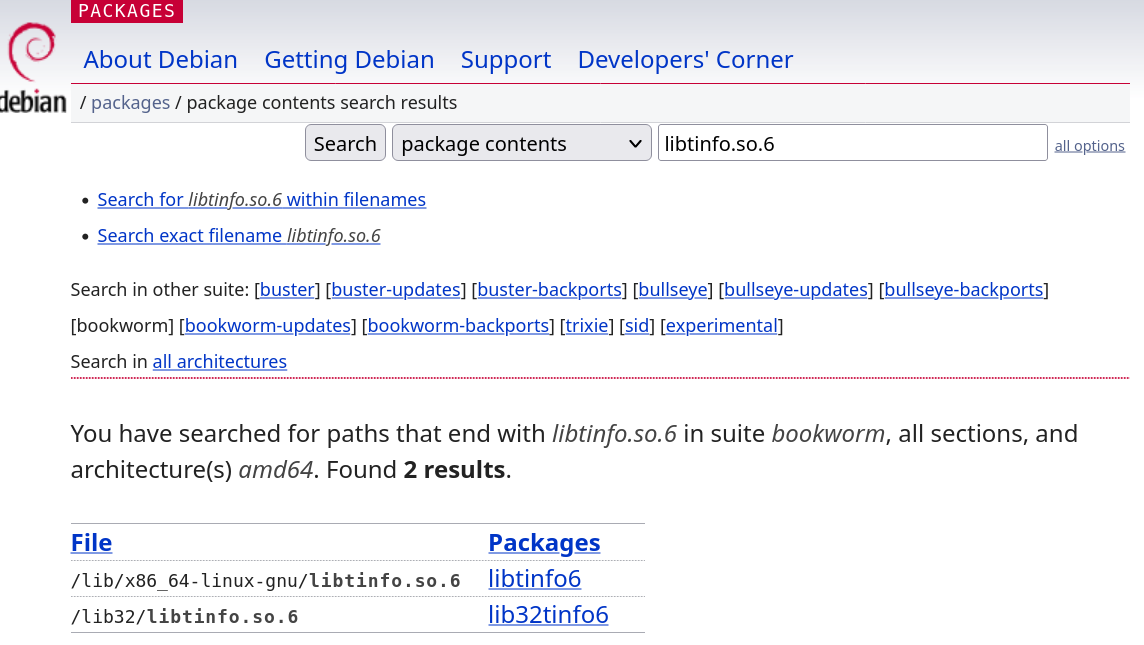
\includegraphics[width=0.7\textwidth]{../re-tools/deb-tinfo1}
\end{frame}

\begin{frame}[fragile]{tinfo? (2)}
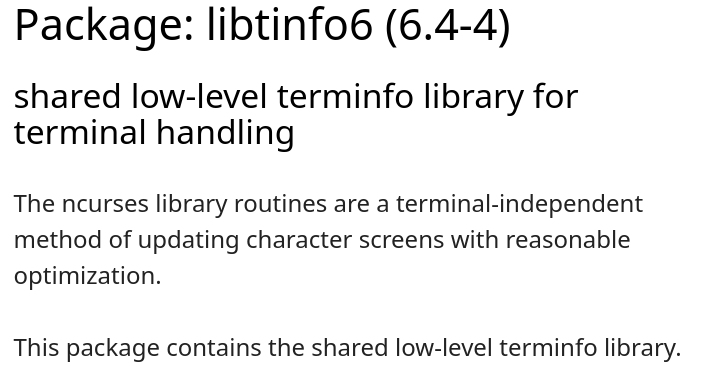
\includegraphics[width=0.7\textwidth]{../re-tools/deb-tinfo2}
\end{frame}

\begin{frame}[fragile]{library calls}
\begin{Verbatim}[fontsize=\fontsize{8}{9}]
$ objdump --dynamic-syms mystery

mystery:     file format elf64-x86-64

DYNAMIC SYMBOL TABLE:
0000000000000000      DF *UND*  0000000000000000 (GLIBC_2.3)  __ctype_toupper_loc
0000000000000000      DF *UND*  0000000000000000 (GLIBC_2.2.5) getenv
0000000000000000      DF *UND*  0000000000000000 (NCURSES6_5.0.19991023) wattrset
0000000000000000      DF *UND*  0000000000000000 (GLIBC_2.2.5) free
0000000000000000      DF *UND*  0000000000000000 (NCURSES6_TINFO_5.0.19991023) flushinp
0000000000000000      DF *UND*  0000000000000000 (GLIBC_2.2.5) localtime
0000000000000000      DF *UND*  0000000000000000 (GLIBC_2.34) __libc_start_main
\end{Verbatim}
\ldots
\begin{Verbatim}[fontsize=\fontsize{9}{10}]
0000000000000000      DF *UND*  0000000000000000 (GLIBC_2.2.5) setuid
\end{Verbatim}
\ldots
\end{frame}

\begin{frame}[fragile]{library calls (Ghidra)}
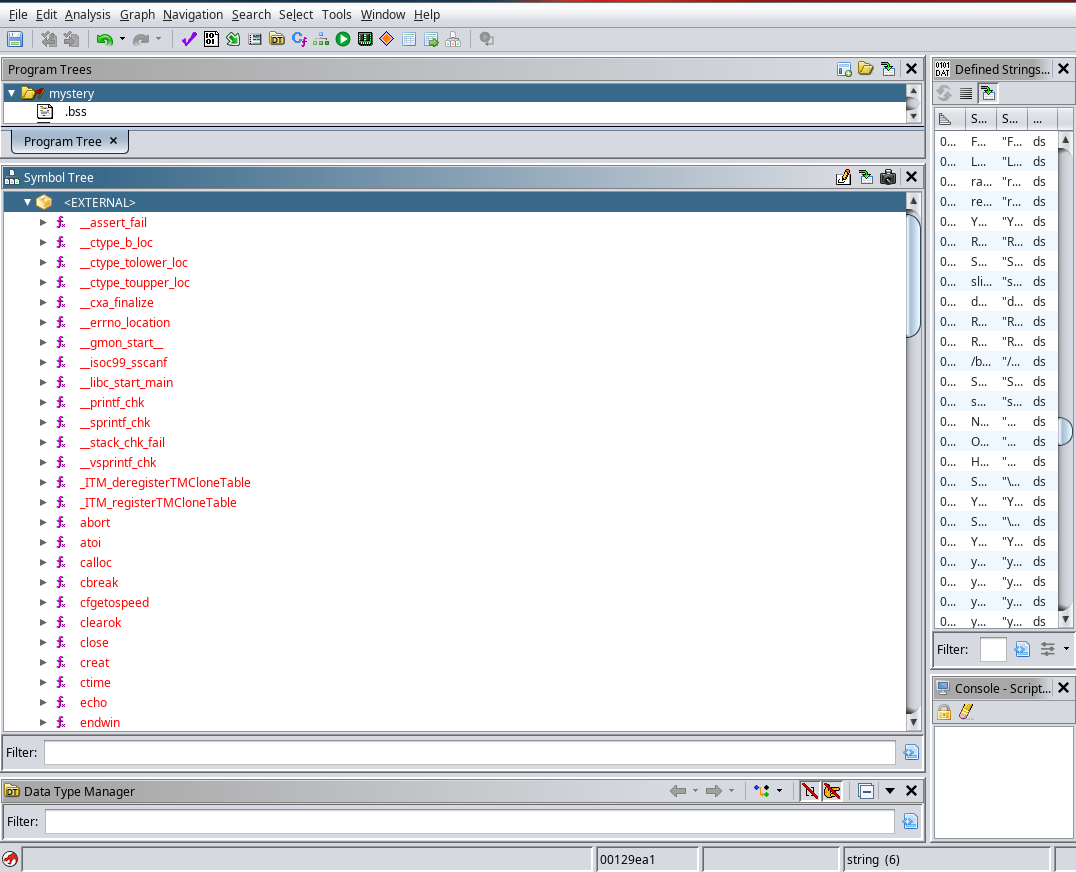
\includegraphics[width=\textwidth]{../re-tools/ghidra-mystery-ext}
\end{frame}

\begin{frame}[fragile]{finding library call uses}
{\small {\tt objdump --disassemble --dyanmic-reloc:}}
\begin{Verbatim}[fontsize=\fontsize{9}{10}]
0000000000005b00 <setuid@plt>:
    5b00:▶      f3 0f 1e fa          ▶  endbr64␣
    5b04:▶      f2 ff 25 fd d3 02 00 ▶  bnd jmp *0x2d3fd(%rip) 
			# 32f08 <setuid@GLIBC_2.2.5>
    5b0b:▶      0f 1f 44 00 00       ▶  nopl   0x0(%rax,%rax,1)
\end{Verbatim}
\ldots
\begin{Verbatim}[fontsize=\fontsize{9}{10}]
   2764f:▶      e8 ec e3 fd ff       ▶  call   5a40 <open@plt>
   27654:▶      89 05 fe 48 01 00    ▶  mov    %eax,0x148fe(%rip)        # 3bf58 <LINES@NCURSES6_TINFO_5.0.19991023+0x5244>
   2765a:▶      31 c0                ▶  xor    %eax,%eax
   2765c:▶      e8 2f e1 fd ff       ▶  call   5790 <getuid@plt>
   27661:▶      89 c7                ▶  mov    %eax,%edi
   27663:▶      31 c0                ▶  xor    %eax,%eax
   27665:▶      e8 96 e4 fd ff       ▶  call   5b00 <setuid@plt>
   2766a:▶      31 c0                ▶  xor    %eax,%eax
   2766c:▶      e8 cf e2 fd ff       ▶  call   5940 <getgid@plt>
   27671:▶      48 83 c4 08          ▶  add    $0x8,%rsp
\end{Verbatim}
\end{frame}

% FIXME: library call uses Ghidra
